\begin{figure}[t]
\centering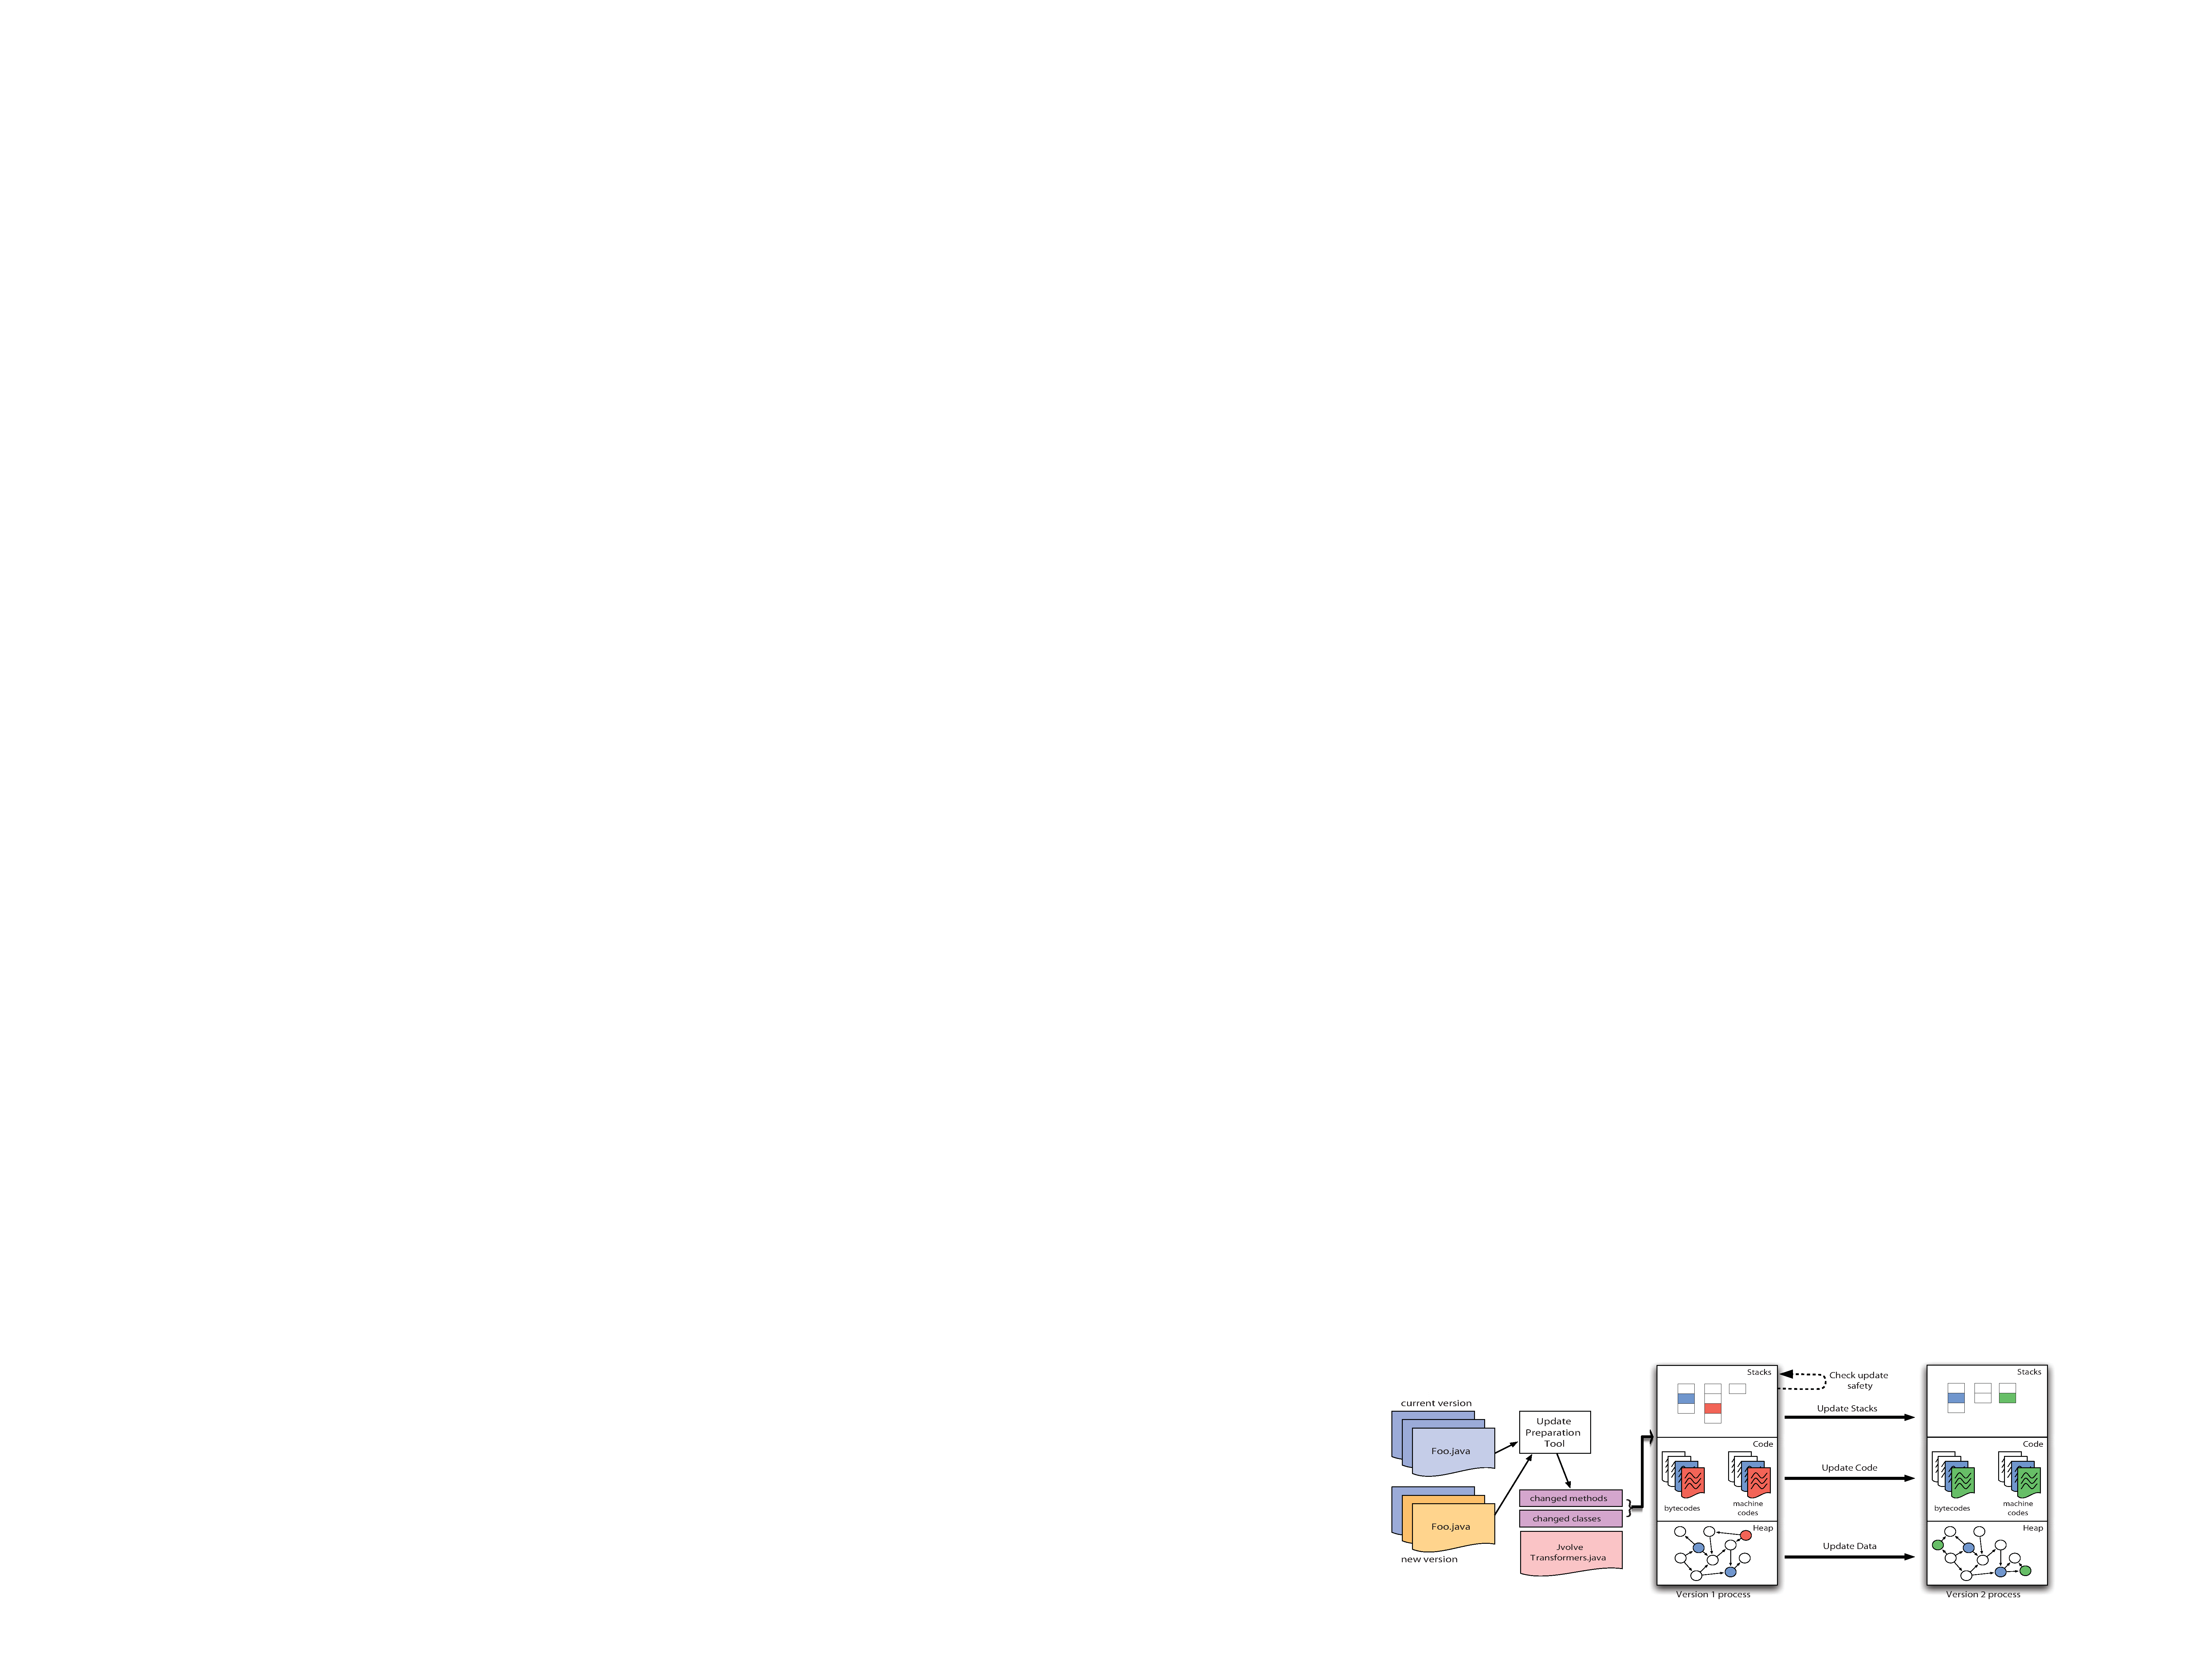
\includegraphics[scale=0.38,clip=true,trim=2170 90 250 2125]{100-images/PASS-HPC-poster-8-2009-cropped}
\caption{Overview of the Dynamic Updating process.\label{fig:overview}}
\end{figure}

\section{Introduction}
\label{sec:system-intro}

Figure~\ref{fig:overview} illustrates the dynamic updating process. The left
portion depicts the work done offline. The developer writes the old and new
versions of the application, and tests them as part of the software
development process. The \acf{UPT} examines source code
of the old and new versions of the application and prepares a dynamic patch.
The user feeds the patch to a process with dynamic-updating support,
depicted on the right. The figure shows two processes, one
running version one of an application, showing stacks, code and heap; and
another running version two of the same application. The goal is to
transition from a process running an old version of the application, to one
running the new version, on the fly, without stopping and restarting the
application.

We assume that developers write and fully test both the old and new
versions using standard development practices without anticipating that
the application is going to be updated dynamically. Testing is already a
well established part of software development. With dynamic updating,
developers should test the update process, in addition to testing their
applications.
When it comes time to
perform the update, the developer provides the source code for the old and
new versions to \JV's \acf{UPT}. The \acs{UPT} compares these two versions
and provides a specification for the update. The specification consists of
two major parts. First, it contains information about code changes that
inform the VM when it is safe to perform the update, what old
methods to invalidate, and what new method bodies to load. Second, it
informs the VM how to deal with changes to data. The VM uses this
specification to transform classes and objects in the heap to conform to
their new version. The programmer has the option to
modify the update specification. Specifically, the
\acs{UPT} does not reason deeply about the semantics of
data structure changes. The programmer may need to modify the \acs{UPT}s
output to obtain a correct program.

Given an update specification, the user
signals the running VM to apply the update.  The VM loads the new class
files and schedules the update. The VM scheduler signals an interrupt, which
stops all threads at VM safe points, where it is safe to perform thread
scheduling and garbage collection. \JV then checks if the VM is at a
\emph{DSU safe point}. DSU safe points require that no thread's activation
stack contains a \emph{restricted} method, which is part of the specification.

Restricted methods are of three categories: (1) methods changed by the
update, (2) methods whose bytecode is unchanged but whose compiled
representation may change, and (3) methods specified by the user or
testing process for semantic reasons. If
restricted methods are on stack, the VM installs return-barriers for~(1)
and~(3), and performs on-stack-replacement for~(2) to reach a DSU safe
point.  Section~\ref{sec:safe} describes how \JV reaches a safe point in
detail.

Once all application threads have synchronized at DSU safe points, \JV
applies the update. It first invalidates the compiled versions of all
changed methods.  These methods are recompiled as needed---the adaptive JIT
compiler will generate code the next time the program invokes an
invalidated method, and will optimize it further, if the program executes it
frequently enough.  The VM then initiates a full copying garbage collection. It
piggybacks on the garbage collector to detect all existing objects whose
classes change. It allocates objects that conform to the new class
definitions.
Finally, after garbage collection, \JV performs class and
object transformations to populate per-class static fields and per-object
instance fields with valid state.  At this point, the update is complete.
